\clearpage

\section {Implementation of $\nu_{e}$-appearance analysis in the {\em VaLOR} analysis framework}
\label{app:standalone}

The analysis presented in this note uses a modified version of the framework used by the 
2012 3-flavour $\nu_{\mu}$-disappearance analysis performed by the Rutherford-Oxford-Lancs group and reported in \cite{OurRun123DisappAnalysis3Flavour}.
One of the main extensions of the framework is the ability to analyze single e-like ring events, a mandatory ingredient for the joint fit. 
This new {\em VaLOR} $\nu_e$-appearance analysis uses the same inputs as the official 2012 $\nu_e$-appearance analysis \cite{NueRun123AnalysisEreco, NueRun123Analysis}.

In order to validate the  {\em VaLOR} $\nu_e$-appearance implementation a comparison with the the official 2012 $\nu_e$-appearance \nolinebreak anal\nolinebreak ysis in \cite{NueRun123AnalysisEreco} 
(the one using reconstructed energy spectrum) will be presented now. For this comparison, the same values of oscillation parameters are used: 
$sin^{2}(2\theta_{12}) = 0.8704$, $\Delta m_{21}^{2} = 7.6 \times 10^{-5}$, $sin^{2}(2\theta_{23}) =  1.0$, $|\Delta m_{32}^{2}| = 2.4 \times 10^{-3}$, $\delta_{CP} = 0$ and normal hierarchy. 

Tables \ref{tab:nueoff1} and \ref{tab:nueoff2} show the predicted number of $\nu_{e}$ candidate events corresponding 
to Run1+2+3 POT for both analyses, before (Table \ref{tab:nueoff1}) and after (Table \ref{tab:nueoff2}) BANFF tuning. 
The agreement is excellent before BANFF tuning, while small differences in Table \ref{tab:nueoff2} are due to different BANFF versions used 
({\em VaLOR}, as explained in \cite{OurRun123DisappAnalysis3Flavour}, is using a more recent BANFF version than the one used for the 2012 official appearance analyses). 



\begin{table}[htbp]
\center
\begin{tabular} {|p{2cm}|p{2.5cm}|p{2.5cm}||p{2.5cm}|p{2.5cm}|}
\hline
Events  & $sin^{2}(2\theta_{13})$ = 0 (official) & $sin^{2}(2\theta_{13})$ = 0  ({\em VaLOR}) & $sin^{2}(2\theta_{13})$ = 0.1 (official) & $sin^{2}(2\theta_{13})$ = 0.1 ({\em VaLOR}) \\
\hline \hline
\textbf{Total}  & \textbf{\color{blue}{3.18}} &\textbf{ 3.175} & \textbf{\color{blue}{11.11}} & \textbf{11.106}  \\
\hline
$\nu_{\mu}$  & \color{blue}{1.21}  & 1.211 & \color{blue}{1.21}  & 1.211   \\
\hline
$\bar{\nu_{\mu}}$  & \color{blue}{0.07} & 0.067 & \color{blue}{0.07}  & 0.067 \\
\hline
$\nu_{e}$  & \color{blue}{1.62} & 1.622 & \color{blue}{1.50} & 1.505 \\
\hline
$\bar{\nu_{e}}$  & \color{blue}{0.08} & 0.083 & \color{blue}{0.08} & 0.079 \\
\hline
osc. $\nu_{e}$ & \color{blue}{0.19}  & 0.192 & \color{blue}{8.24}  & 8.245 \\
\hline
\end{tabular}
\caption{Predicted number of $\nu_{e}$ candidate events for the Run1+2+3 POT before BANFF tuning (that is, after external flux reweighting 
using default 11c SK MC with the 11b tuned version 3.2), for {\em VaLOR} appearance 
analysis (black) compared to official appearance analysis (blue) as in Table 1 of \cite{NueRun123AnalysisEreco}, 
using $sin^{2}(2\theta_{12}) = 0.8704$, $\Delta m_{21}^{2} = 7.6 \times 10^{-5}$, 
$sin^{2}(2\theta_{23}) =  1.0$, $|\Delta m_{32}^{2}| = 2.4 \times 10^{-3}$, $\delta_{CP} = 0$ and normal hierarchy.}
\label{tab:nueoff1}
\end{table}

\begin{table}[htbp]
\center
\begin{tabular} {|p{2cm}|p{2.5cm}|p{2.5cm}||p{2.5cm}|p{2.5cm}|}
\hline
Events  & $sin^{2}(2\theta_{13})$ = 0 (official) & $sin^{2}(2\theta_{13})$ = 0  ({\em VaLOR}) & $sin^{2}(2\theta_{13})$ = 0.1 (official) & $sin^{2}(2\theta_{13})$ = 0.1 ({\em VaLOR}) \\
\hline \hline
\textbf{Total}  & \textbf{\color{blue}{3.29}} &\textbf{ 3.210}          & \textbf{\color{blue}{11.19}} & \textbf{11.052}  \\
\hline
$\nu_{\mu}$  & \color{blue}{1.18}  & 1.163          & \color{blue}{1.18}  & 1.163   \\
\hline
$\bar{\nu_{\mu}}$  & \color{blue}{0.07} & 0.065         & \color{blue}{0.07}  & 0.065 \\
\hline
$\nu_{e}$  & \color{blue}{1.75} & 1.703            & \color{blue}{1.63} & 1.581 \\
\hline
$\bar{\nu_{e}}$  & \color{blue}{0.09} & 0.089           & \color{blue}{0.09} & 0.084 \\
\hline
osc. $\nu_{e}$ & \color{blue}{0.19}  & 0.189          & \color{blue}{8.23}  & 8.158 \\
\hline
\end{tabular}
\caption{Predicted number of $\nu_{e}$ candidate events for the Run1+2+3 POT after applying BANFF tuning (post ND280 fitted values) 
for {\em VaLOR} appearance analysis (black) compared to official appearance analysis (blue) 
as in Table 9 of \cite{NueRun123AnalysisEreco},using  $sin^{2}(2\theta_{12}) = 0.8704$, 
$\Delta m_{21}^{2} = 7.6 \times 10^{-5}$, $sin^{2}(2\theta_{23}) =  1.0$, $|\Delta m_{32}^{2}| = 2.4 \times 10^{-3}$, $\delta_{CP} = 0$ and normal hierarchy. }
\label{tab:nueoff2}
\end{table}

Fig.~\ref{fig:nueoff1} presents the MC predicted reconstructed neutrino energy distribution (area-normalized) for $\nu_{\mu} \rightarrow \nu_{e}$ CC signal, 
intrinsic $\nu_{e}$ CC background and NC background components 
obtained with the {\em VaLOR} framework, in excellent agreement with Fig. 1 in \cite{NueRun123AnalysisEreco} for the official appearance analysis. 

\begin{figure}[htbp]
\begin{center}
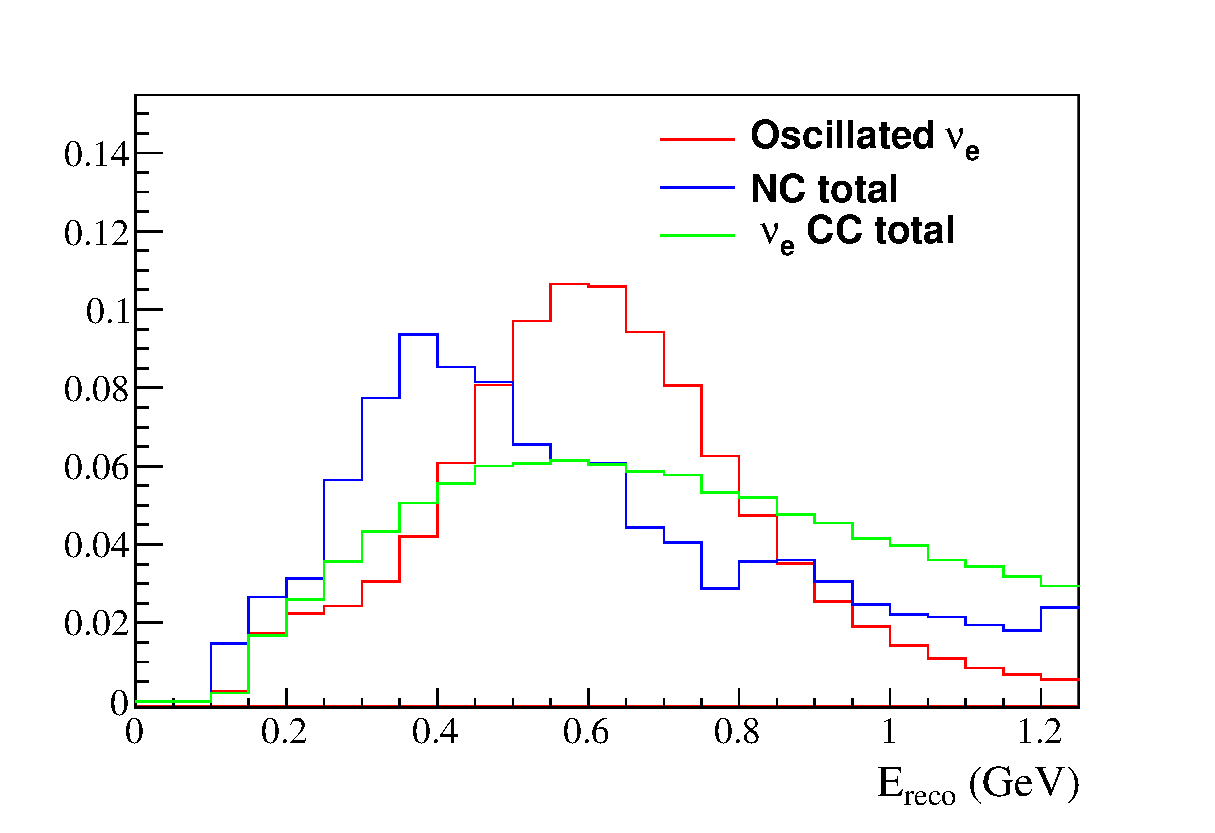
\includegraphics[width=0.5\textwidth]{images/appendix/nue_standalone/ErecoDistForComparisonFig1Nakayama.eps}
\caption{MC predicted reconstructed neutrino energy distribution (area-normalized) for $\nu_{\mu} \rightarrow \nu_{e}$ CC signal (red), intrinsic $\nu_{e}$ CC background (green) 
and NC background (blue) components obtained with {\em VaLOR} framework, using  
$sin^{2}(2\theta_{12}) = 0.8704$, $\Delta m_{21}^{2} = 7.6 \times 10^{-5}$, 
$sin^{2}(2\theta_{23}) =  1.0$, $|\Delta m_{32}^{2}| = 2.4 \times 10^{-3}$, $\delta_{CP} = 0$ and normal hierarchy. }
\label{fig:nueoff1}
\end{center}
\end{figure}

A p-value test similar to the one described in \cite{NueRun123AnalysisEreco} has been performed. 11 $\nu_{e}$ candidates has been observed in the Run1+2+3 data-set. 
The p-value is defined as the probability for observing 11 or more $\nu_{e}$ candidate events in the $3.010 \times 10^{20}$ POT data with the $sin^{2}(2\theta_{13}) = 0$ hypothesis.  
$1 \times 10^{6}$ toy experiments with statistical and systematic variations were created in order to compute that probability. 
Fig.~\ref{fig:nueoffpvalue} shows the distribution of the number of $\nu_{e}$ candidate events observed. 
The p-value, corresponding to the area above 11 (white region), is $\approx 8 \times 10^{-4}$, equivalent to a $\approx 3\sigma$ significance. These values, 
although computed with 100 times less toy experiments, are very close to the ones obtained in \cite{NueRun123AnalysisEreco} 
(p-value = $8.6 \times 10^{-4}$, $3.1\sigma$ significance). 

\begin{figure}[htbp]
\center
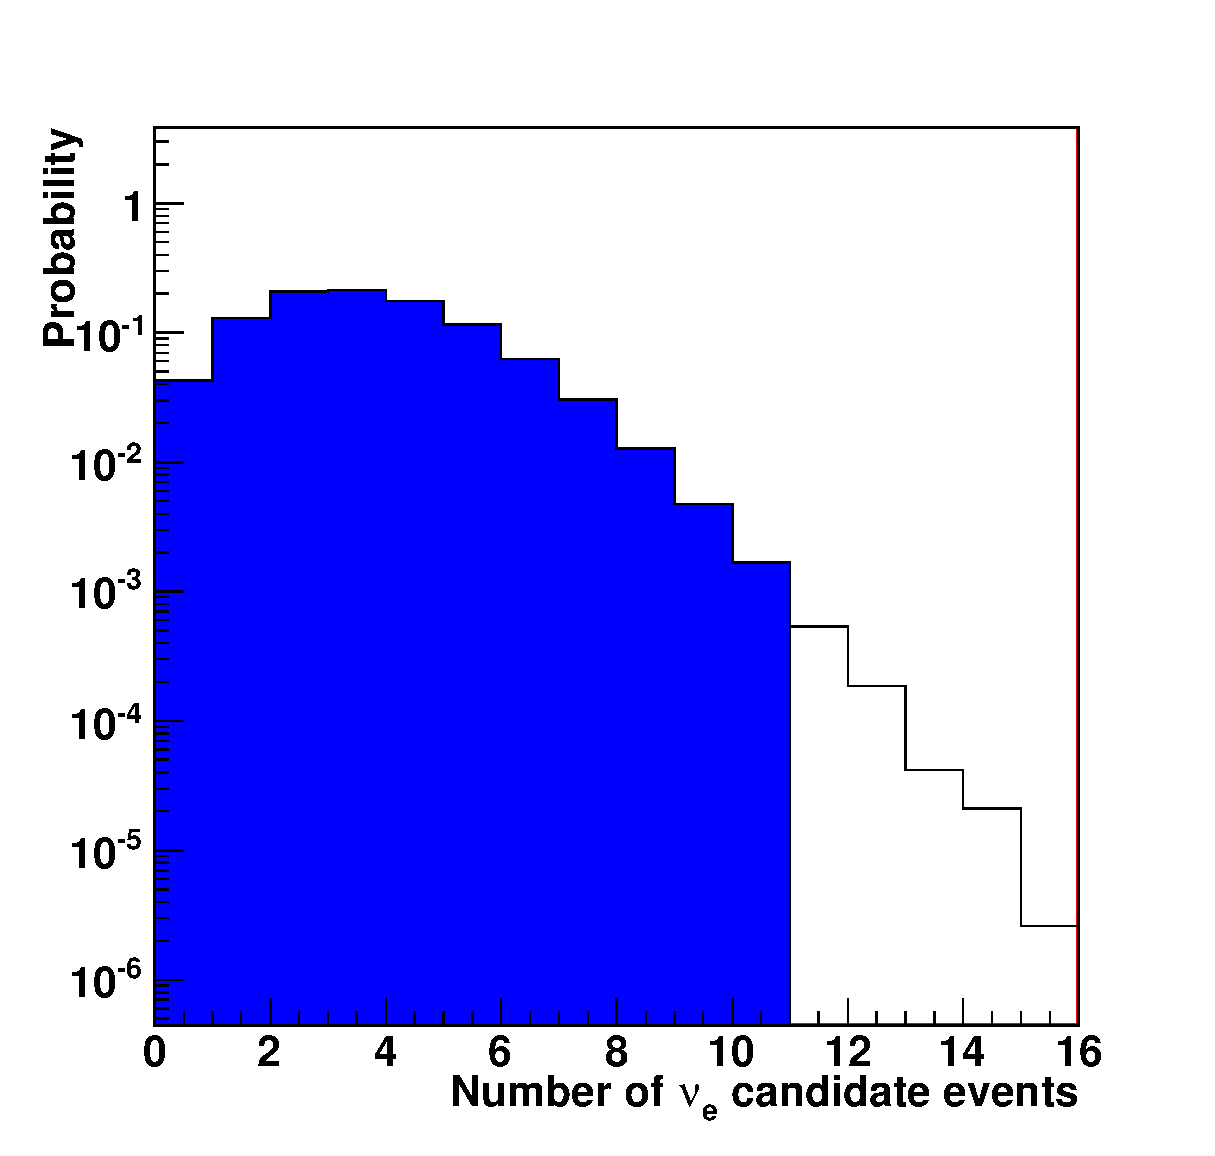
\includegraphics[width=0.5\textwidth]{images/appendix/nue_standalone/PValue.eps}
\caption{ Distribution of predicted number of $nu_{e}$ candidate events over $1\times10^{6}$ toy experiments with $sin^{2}(2\theta_{13}) =  0$, including statistical and systematic variations, for  $3.010 \times 10^{20}$ POT,
$sin^{2}(2\theta_{12}) = 0.8704$, $\Delta m_{21}^{2} = 7.6 \times 10^{-5}$, $sin^{2}(2\theta_{23}) =  1.0$, $|\Delta m_{32}^{2}| = 2.4 \times 10^{-3}$, $\delta_{CP} = 0$ and normal hierarchy. }
\label{fig:nueoffpvalue}
\end{figure}


The fit to the Run1+2+3 data-set is the next step in the validation. Fig.~\ref{fig:nueoff2} shows the $\Delta\chi^{2}$ curve for normal (left) and inverted (right) hierarchy, 
in great agreement with Fig. 20 in \cite{NueRun123AnalysisEreco}.
The corresponding best-fit point and confidence intervals for $sin^{2}(2\theta_{13})$ are summarized in table \ref{tab:nueoff3}. 
Finally, the reconstructed energy spectrum at the best-fit point is presented in Fig.~\ref{fig:nueoff3}, 
which is again in excellent agreement with Fig. 21 in \cite{NueRun123AnalysisEreco}. 

From these comparisons and other detailed tests not shown here, it is concluded that the 2012 {\em VaLOR} stand-alone $\nu_e$-appearance 
analysis gives equivalent results to the T2K official appearance analyses.


\begin{figure}[htbp]
\center
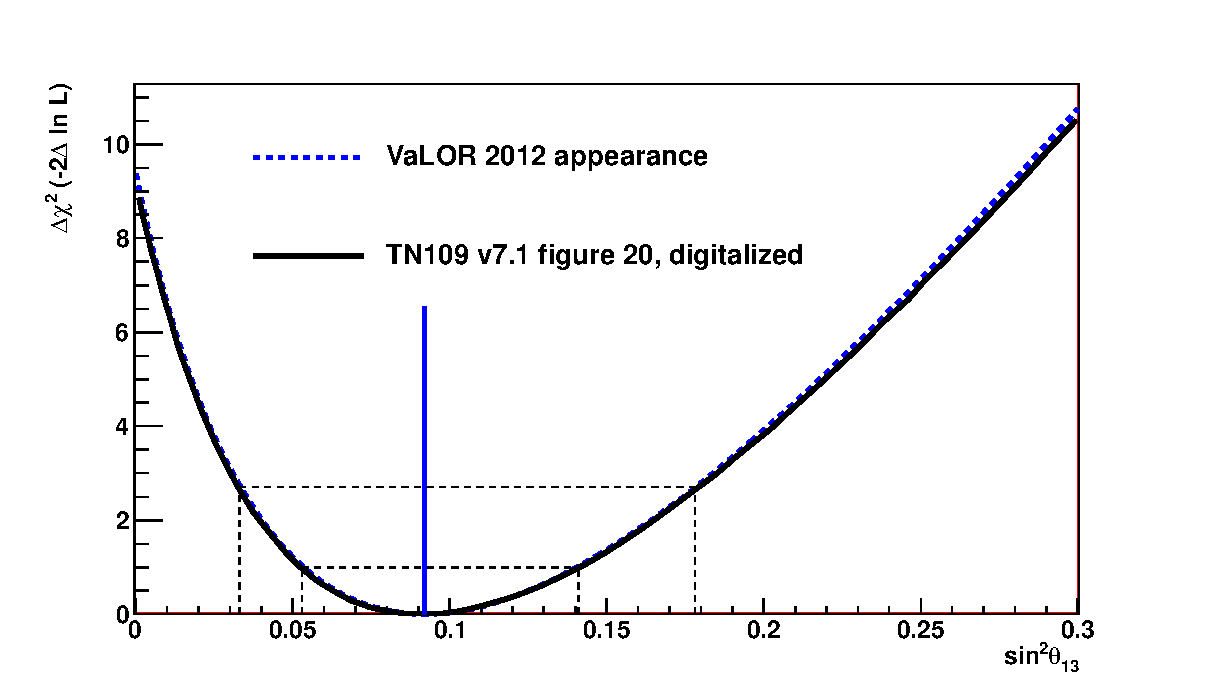
\includegraphics[width=0.5\textwidth]{images/appendix/nue_standalone/OffNue2012DeltaChisqNH.eps}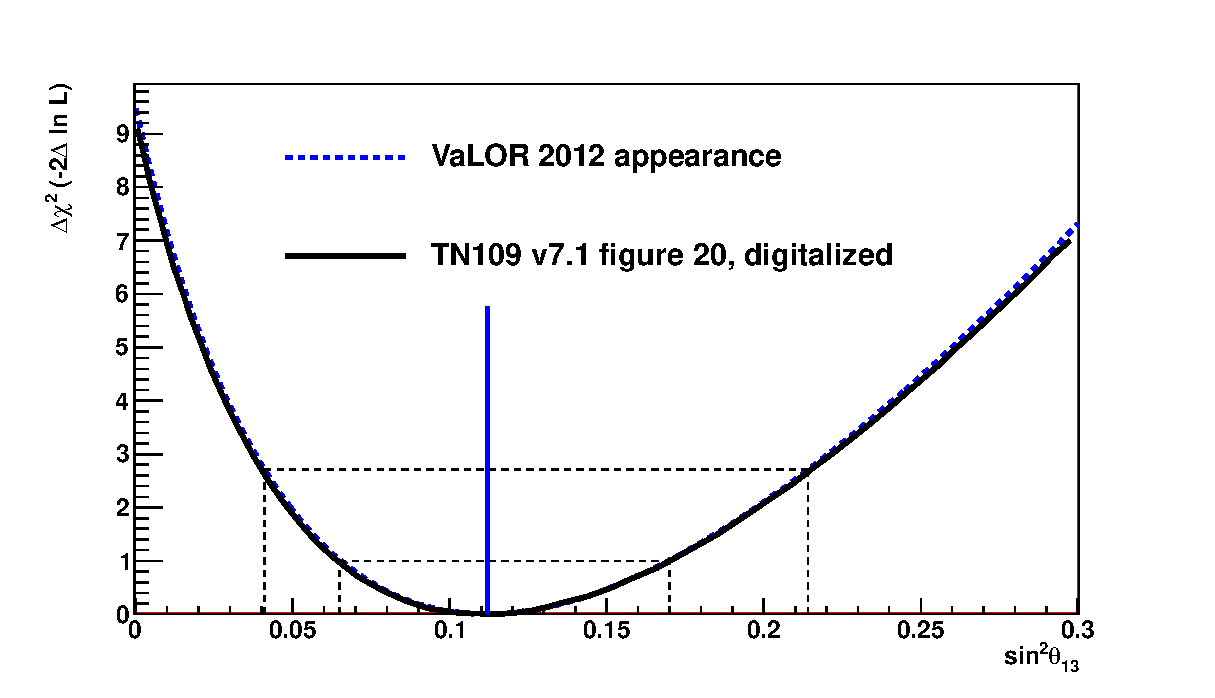
\includegraphics[width=0.5\textwidth]{images/appendix/nue_standalone/OffNue2012DeltaChisqIH.eps}
\caption{$\Delta\chi^{2}$ distribution for the Run1+2+3 data fit assuming normal (left) and inverted (right) mass hierarchy, for 2012 {\em VaLOR} appearance analysis (dashed blue) and 2012 
official results from Fig. 21 in \cite{NueRun123AnalysisEreco} (solid black - digitalized). Fixed values used: $sin^{2}(2\theta_{12}) = 0.8704$, 
$\Delta m_{21}^{2} = 7.6 \times 10^{-5}$, $sin^{2}(2\theta_{23}) =  1.0$, $|\Delta m_{32}^{2}| = 2.4 \times 10^{-3}$ and $\delta_{CP} = 0$.}
\label{fig:nueoff2}
\end{figure}



\begin{table}[htbp]
\center
\begin{tabular}{|c|c|c|c|c|}
\hline 
 & NH (TN109) & NH ({\em VaLOR}) & IH (TN109) & IH ({\em VaLOR}) \\
 \hline \hline
 Best fit & \color{blue}{0.092} & 0.092 & \color{blue}{0.112} & 0.112 \\
  \hline
  68 \% C.L. & \color{blue}{0.053-0.141} & 0.053-0.141&  \color{blue}{ 0.065-0.170} &  0.065 - 0.170\\
  \hline
    90 \% C.L. & \color{blue}{0.033-0.179} & 0.033-0.178 &  \color{blue}{ 0.040-0.215} & 0.041 - 0.214 \\
\hline
\end{tabular}
\caption{Best-fit points and confidence intervals for $sin^{2}(2\theta_{13})$ obtained from Fig.~\ref{fig:nueoff2}, 
with $\delta_{CP} = 0$, $sin^{2}(2\theta_{12}) = 0.8704$, $\Delta m_{21}^{2} = 7.6 \times 10^{-5}$, 
$sin^{2}(2\theta_{23}) =  1.0$ and $|\Delta m_{32}^{2}| = 2.4 \times 10^{-3}$, for normal (NH) and inverted (IH) hierarchy. }
\label{tab:nueoff3}
\end{table}



\begin{figure}[htbp]
\center
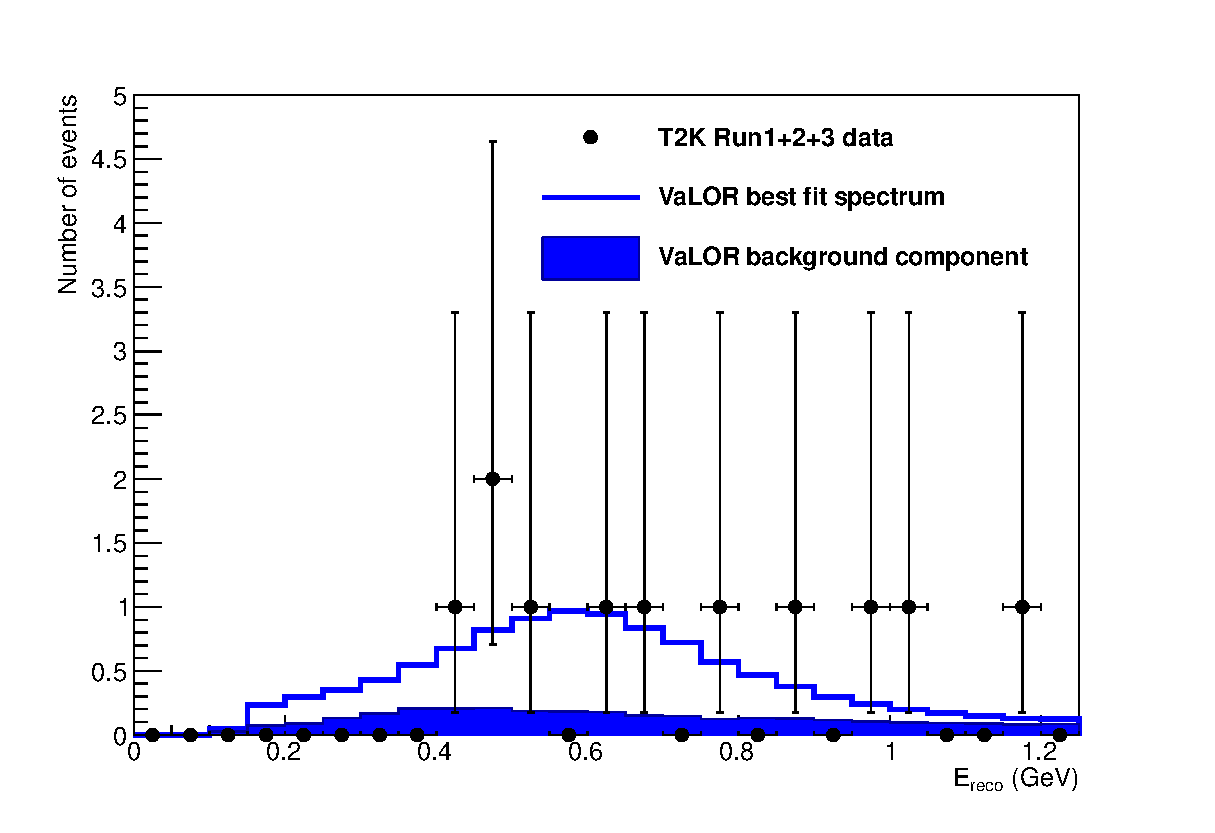
\includegraphics[width=0.5\textwidth]{images/appendix/nue_standalone/BestFitData2012NH.eps}
\caption{Reconstructed energy spectrum at the best-fit point for Run1+2+3 data fit with the {\em VaLOR} 
appearance analysis, 
assuming $\delta_{CP} = 0$, $sin^{2}(2\theta_{12}) = 0.8704$, $\Delta m_{21}^{2} = 7.6 \times 10^{-5}$, $sin^{2}(2\theta_{23}) =  1.0$, $|\Delta m_{32}^{2}| = 2.4 \times 10^{-3}$ and normal hierarchy.}
\label{fig:nueoff3}
\end{figure}




%is presented in Fig.\ \ref{fig:nuecomparison}. 
%The numbers of signal and background events obtained from the two analyses are compared in table \ref{tab:nueoff} 
%for two different values of $\sin^{2}2\theta_{13}$.
%From these comparisons and other detailed tests not shown here, we conclude that the {\em VaLOR} $\nu_e$-appearance 
%analysis gives equivalent results to the T2K official analyses.

%\begin{figure}[htbp]
%\begin{center}
%\includegraphics[width=0.8\textwidth]{images/appendix/ConfidenceContoursNueNormal.eps}
%\caption{Comparison of 90\% (blue) and 68\% (red) C.L. contours from the T2K official $\nu_{e}$-appearance analysis \cite{NueRun1and2Analysis} 
    %    (dashed lines, light colors) with those obtained with the {\em VaLOR} $\nu_{e}$-appearance analysis (solid lines, dark colors). The {\em VaLOR} 
        %contours are in good agreement with those from the  official analysis; the small differences are due to the limited number of 
        %Feldman-Cousins jobs run for this comparison.}
%\label{fig:nuecomparison}
%\end{center}
%\end{figure}

%\begin{table}[h]
%\centering
%\begin{tabular}{|c|c|c|c|c|}
%\hline
 % & \multicolumn{2}{|c|}{$\sin^{2}2\theta_{23}$ = 0} & \multicolumn{2}{|c|}{$\sin^{2}2\theta_{23}$ = 0.1} \\
%\cline{2-5}
 % & T2K official & {\em VaLOR}  & T2K official & {\em VaLOR} \\
%\hline \hline
%Beam total & 1.40 & 1.44 & 1.34 & 1.37 \\
%\hline
%Beam $\nu_{\mu}$ and $\bar{\nu_{\mu}}$ CC  & 0.03 & 0.03 & 0.03 & 0.03 \\
%Beam $\nu_{e}$ CC  & 0.76 & 0.77 & 0.70 & 0.71 \\
%all NC  & 0.61 & 0.63 & 0.61 & 0.63 \\
%\hline
%Signal $\nu_{\mu}\rightarrow\nu_{e}$  & 0.09 & 0.09 & 4.11 & 4.18 \\
%\hline
%Total & 1.49 & 1.53 & 5.45 & 5.55 \\
%\hline
%\end{tabular}
%\caption{Comparison of numbers of $\nu_{e}$ events in SuperK at $\sin^{2}2\theta_{13}=0$ and $\sin^{2}2\theta_{13}=0.1$ between the T2K 
   %      official analysis \cite{NueRun1and2Analysis} and the {\em VaLOR} stand-alone $\nu_{e}$-appearance analysis.}
%\label{tab:nueoff}
%\end{table}



% continuation of the analyses performed by the same group on the 2-flavour $\nu_{\mu}$-disappearance framework described in Ref. \cite{OurRun1and2Analysis2F}, \cite{OurRun1DisappAnalysis2F}. The different inputs used for this joint oscillation analysis, corresponding to the T2K 2010 analysis, that are not specified in this section are described in Ref. \cite{OurRun1and2Analysis2F} and \cite{OurRun1DisappAnalysis2F}.

% A full 3-flavour framework with matter effects was implemented by the Rutherford-Oxford-Lancs group as reported in Ref. \cite{OurRun1and2Analysis3F}. In the same framework, the elements to build also the $\nu_{e}$-appearance analysis were included, following the descriptions in Ref.\cite{NueRun1and2Analysis}, becoming the {\em VaLOR} framework for the joint oscillation analysis which handles the 1R$\mu$ sample and the 1Re sample at the same time. Details about the stand-alone appearance and disappearance analyses combined for the joint analysis will be described in this section.

% \subsection{Event selection cuts}

% The nominal SuperK one ring e-like and $\mu$-like MC templates are constructed by applying the one ring e-like or $\mu$-like selection cuts on the official SuperK MC samples. The \textbf{one ring e-like selection cuts} correspond to the official 2010 cuts that can be summarized as follows:

% \begin{enumerate}
% \item{Fully contained: the number of PMT hits in highest-charge OD cluster is less than 16. }
% \item{Fiducial volume: the reconstructed vertex is at least 2m away from ID wall.}
% \item{Visible energy cut: the visible energy in the event is above 100 MeV ($E_{vis}>100MeV$).}
% \item{One ring cut: there is only one reconstructed ring in the event.}
% \item{PID cut: the reconstructed ring is e-like (ip[0]=2).}
% \item{Michel electron cut: the number of decay electrons must be 0.}
% \item{Pi0 mass cut: the invariant mass calculated with forced second ring is less than 105MeV ($M_{inv}<105 MeV$).}
% \item{Reconstructed neutrino energy cut: the reconstructed neutrino energy is less than 1250 MeV ($E_{\nu}^{reco}<1250MeV$).}
% \end{enumerate}

% The \textbf{one ring $\mu$-like selection cuts} also correspond to the official 2010 cuts and are the following ones:

% \begin{enumerate}
% \item{Fully contained: the number of PMT hits in highest-charge OD cluster is less than 16. }
% \item{Fiducial volume: the reconstructed vertex is at least 2m away from ID wall.}
% \item{Visible energy cut: the visible energy in the event is above 30 MeV ($E_{vis}>30MeV$).}
% \item{One ring cut: there is only one reconstructed ring in the event.}
% \item{PID cut: the reconstructed ring is $\mu$-like (ip[0]=3).}
% \item{Muon momentum cut: the momentum reconstructed as muon must be larger than 200 MeV (amomm[0]$>$200MeV)}
% \item{Michel electron cut: the number of decay electrons must be no larger than one ($<=1$ decay $e^{-}$).}
% \end{enumerate}


% \subsection{SK MC templates and prediction}

% For the new \textbf{1R$_{e}$-like sample} the following NEUT interaction modes were included: 

% \begin{enumerate}
% \item{CCQE, CC1$\pi$, CC coh and CC other for $\nu_{\mu}$, $\overline{\nu_{\mu}}$ and $\nu_{e}$}
% \item{NC1$\pi$0, NC coh and NC other for $\nu_{\mu}$, $\overline{\nu_{\mu}}$ and $\nu_{e}$}
% \item{ CCQE, CC1$\pi$ and CC other for signal $\nu_{e}$}
% \end{enumerate}

%  The interaction modes used for the \textbf{1R$_{\mu}$-like sample} were: 
%  \begin{enumerate}
%  \item{CCQE, CC1$\pi$, CC other and NC for $\nu_{\mu}$, $\overline{\nu_{\mu}}$ and $\nu_{e}$}
%  \item{ CCQE, CC1$\pi$ and CC other for signal $\nu_{e}$}
%  \end{enumerate}
 
% In general, the NC modes for signal $\nu_{e}$ are not used, and the NC modes for the rest of flavours are not oscillated (oscillation probabilities set to 1 for them). Notice that the CC other definition is different for the 1R$_{\mu}$ and 1R$_{e}$ samples: in the 1R$_{\mu}$ the CC coh. mode is included in the CC other category while for 1R$_{e}$ is not. The list of interaction modes considered will be updated in next joint analysis, with 2012 upgrades.
 
% For the mu-like sample the $E_{reco}$ spectrum will be used, while for the e-like sample only the number of events (the integral of the $E_{reco}$ spectrum) will be used. In both cases, the steps to construct the SK prediction from the SK MC templates just defined can be summarized as follows:

% \begin{enumerate}
% \item The SK MC files contain for the events passing all cuts previously defined a small ntuple with the following variables : reconstructed energy (erec or EnuReco), generator interaction mode, neutrino true energy (Etrue or inu) and the flavour identification (pdg or ipnu).
% \item With this SK MC files, for each neutrino flavour and mode a SK MC template is filled with the number of events in two dimensional ($E_{reco}$,$E_{true}$) bins. 
% \item A first reweighting is applied to these samples: the number of events is weighted in each ($E_{reco}$,$E_{true}$) bin by (data POT / MC POT) depending on the interaction mode and neutrino flavour.
% \item Then, multiplicative systematic errors are applied to all templates, reweighting the number of events in each ($E_{reco}$,$E_{true}$) bin. These multiplicative systematics can be dependent on the neutrino true or reconstructed energy and they are: flux shape, efficiencies, cross sections and FSI systematics. The flux reweighting (flux version 10a $\rightarrow$ 10d) is applied along with these systematic errors. 
% \item With all multiplicative systematic errors included now the reconstructed energy scale systematic is applied to all templates. This systematic error is applied scaling the edges of the $E_{reco}$ bins and calculating the number of events that each bin has gained and/or lost from adjacent bins assuming a uniform distribution of events in each bin.
% \item Now the neutrino oscillations are applied to the templates with systematics already included. The oscillation probabilities are calculated for the different neutrino flavours depending on the true neutrino energy and the input value of the oscillation parameters, and then applied to the corresponding template (according to its flavour) and ($E_{reco}$,$E_{true}$) bin. 
% \item Finally a sum over all $E_{true}$ bins is performed in each template to construct the $E_{reco}$ spectrum for each neutrino flavour and mode. 
% \item A total $E_{reco}$ spectrum is built adding the content in the same $E_{reco}$  bin for all modes and flavours histograms. The number of events for the 1R$_{e}$-like sample is the integral of the total $E_{reco}$ spectrum.
%  \end{enumerate} 

% \subsection{Systematic errors}

% For the $\nu_{\mu}$-disappearance analysis, the list of systematic errors included in the analysis, described in Ref. \cite{OurRun1and2Analysis2F} and  \cite{OurRun1DisappAnalysis2F}, is the following:

% \begin{enumerate}
% \item SuperK CCQE efficiency
% \item SuperK CCnonQE efficiency
% \item SuperK NC efficiency
% \item Super $\nu_{e}$ CC efificiency
% \item SuperK ring counting
% \item ND280 efficiency
% \item Flux normalization
% \item Flux shape
% \item FSI
% \item SuperK energy scale
% \item CCQE cross section
% \item CC$1\pi$/CCQE cross section ratio
% \item NC/CCQE cross section ratio
% \item CCother/CCQE cross section ratio
% \item NC/CCQE cross section ratio
% \end{enumerate}

% Some of the systematics already mentioned at fully correlated for both the one ring e-like and one ring $\mu$-like samples so they are common for both of them in the joint oscillation analysis:

% \begin{enumerate}
% \item SuperK ring counting
% \item SuperK energy scale
% \item CCQE cross section
% \item CC$1\pi$/CCQE cross section ratio
% \item CCother/CCQE cross section ratio
% \item FSI
% \item ND280 normalization
% \item Flux normalization
% \end{enumerate}

% Additionally to the systematic uncertainties already mentioned, several other systematic parameters only related to the one ring e-like sample were included. They can be summarized as follows:

% \begin{enumerate}
% \item 1Re-like signal SuperK efficiency 
% \item 1Re-like background SuperK efficiency 
% \item CC coh. to CCQE cross section 
% \item NC 1$\pi^{0}$ to CCQE cross section 
% \item NC coh. to CCQE cross section
% \item NC other to CCQE cross section 
% \item $\nu_{e}$ to $\nu_{\mu}$ cross section
% \end{enumerate}

% The uncertainties on the cross sections were provided by the NIWG and are obtained from the version file niwg\_errors\_10a\_v1.root.
% One sigma uncertainties of the systematic parameters related to SuperK detector efficiency for signal (1.4\%) and background (1.4\%) events are taken from \cite{NueRun1and2Analysis}, coming in turn from Table 24 in \cite{TN28}.
% The effect of specific systematics for the $\nu_{e}$-appearance analysis introduced was checked in comparison with the results available (in Ref. \cite{NueRun1and2Analysis}, table 3).


% \subsection{Validation of the stand-alone appearance analysis}

% Once the updates and additions were introduced and operative, the first natural step was to reproduce the official results for the $\nu_{e}$-appearance contours reported in Ref.\cite{NueRun1and2Analysis}. Figure \ref{fig:nuecomparison} shows the comparison of the 68\% and 90\% C.L. contours of the $\nu_{e}$-appearance analysis done with the framework used in this work and the official results, taken from \cite{OfficialNueAnalysisCodeT2KWebsite}. The preliminary results are in very good agreement with the official analysis, small differences appear due to the limited number of Feldman-Cousins jobs \cite{FeldmanCousins} run for this comparison intended to be a quick check. Table \ref{tab:nueoff} shows a comparison between the number of events at $sin^{2}2\theta_{13}=0$ and $sin^{2}2\theta_{13}=0.1$ for the different beam components and signal for the official analysis (taken from Table 16 in \cite{NueRun1and2Analysis}) and the stand-alone study done for this work. 

% \begin{figure}[htbp]
% \begin{center}
% \includegraphics[width=0.8\textwidth]{images/appendix/ConfidenceContoursNueNormal.eps}
% \caption{Comparison of 90\% (blue) and 68\% (red) C.L. contours for the official $\nu_{e}$-appearance analysis \cite{NueRun1and2Analysis} (dashed, light colors)  and the ones obtained with the framework used in this work (solid, dark colors). The new contours are in good agreement with the official ones, small differences appear due to the limited number of FC jobs run for this comparison.}
% \label{fig:nuecomparison}
% \end{center}
% \end{figure}

% \begin{table}[h]
% \centering
% \begin{tabular}{|c|c|c|c|c|}
% \hline
%   & $sin^{2}2\theta_{23}=0$ official & $sin^{2}2\theta_{23}=0$ & $sin^{2}2\theta_{23}=0.1$ official & $sin^{2}2\theta_{23}=0.1$\\
% \hline \hline
% Beam total & 1.40 & 1.44 & 1.34 & 1.37 \\
% \hline
% Beam $\nu_{\mu}$ and $\bar{\nu_{\mu}}$ CC  & 0.03 & 0.03 & 0.03 & 0.03 \\
% Beam $\nu_{e}$ CC  & 0.76 & 0.77 & 0.70 & 0.71 \\
% all NC  & 0.61 & 0.63 & 0.61 & 0.63 \\
% \hline
% Signal $\nu_{\mu}\rightarrow\nu_{e}$  & 0.09 & 0.09 & 4.11 & 4.18 \\
% \hline
% Total & 1.49 & 1.53 & 5.45 & 5.55 \\
% \hline
% \end{tabular}
% \caption{ Comparison of number of events at $sin^{2}2\theta_{13}=0$ and $sin^{2}2\theta_{13}=0.1$ for the different beam components and signal for the official analysis and the stand-alone study done for this work. }
% \label{tab:nueoff}
% \end{table}


